
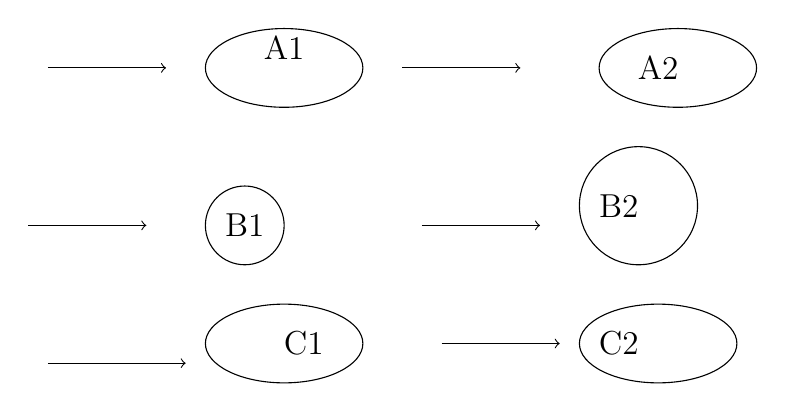
\begin{tikzpicture}
    \tikzstyle{every node}=[font=\large]
    
    % Row 1 (A1 to A2)
    \draw [->] (1.5,16.75) -- (3,16.75);
    \draw  (4.5,16.75) ellipse (1cm and 0.5cm);
    \draw [->] (6,16.75) -- (7.5,16.75);
    \draw  (9.5,16.75) ellipse (1cm and 0.5cm);
    \node at (4.5,17) {A1};
    \node at (9.25,16.75) {A2};

    % Row 2 (B1 to B2)
    \draw [->] (1.25,14.75) -- (2.75,14.75);
    \draw [->] (6.25,14.75) -- (7.75,14.75);
    \draw  (4,14.75) circle (0.5cm);
    \draw  (9,15) circle (0.75cm);
    \node at (4,14.75) {B1};
    \node at (8.75,15) {B2};

    % Row 3 (C1 to (1.5,13) -- (3.25,13);
    \draw [->] (1.5,13) -- (3.25,13);
    \draw  (4.5,13.25) ellipse (1cm and 0.5cm);
    \draw [->] (6.5,13.25) -- (8,13.25);
    \draw  (9.25,13.25) ellipse (1cm and 0.5cm);
    \node at (4.75,13.25) {C1};
    \node at (8.75,13.25) {C2};

\end{tikzpicture}
